\documentclass[11pt,a4paper,landscape]{article}
\usepackage[margin=0.5in]{geometry}
\usepackage{booktabs}
\usepackage{array}
\usepackage{xcolor}
\usepackage{colortbl}
\usepackage{adjustbox}
\usepackage{multirow}
\usepackage{graphicx}
\usepackage{tikz}
\usepackage{fontspec}
\usepackage[default,scale=0.95]{opensans}

% Define ENBEL color scheme
\definecolor{enbelblue}{RGB}{0,83,155}
\definecolor{enbelorange}{RGB}{255,127,0}
\definecolor{enbelgreen}{RGB}{44,160,44}
\definecolor{enbelpurple}{RGB}{148,103,189}
\definecolor{enbelred}{RGB}{214,39,40}
\definecolor{enbelgray}{RGB}{140,140,140}
\definecolor{lightgray}{RGB}{245,245,245}
\definecolor{darkgray}{RGB}{80,80,80}

\pagestyle{empty}

\begin{document}

\begin{center}
{\LARGE \color{enbelblue}\textbf{Key Climate-Health Associations}}\\[0.5em]
{\large \color{darkgray}Novel Findings from Urban African Cohort (N = 18,205)}
\end{center}

\vspace{1em}

\begin{adjustbox}{width=\textwidth,center}
\renewcommand{\arraystretch}{1.5}
\begin{tabular}{@{}l>{\raggedright}p{3.5cm}ccccp{4.5cm}@{}}
\toprule
\rowcolor{enbelblue}
\textcolor{white}{\textbf{Biomarker}} & 
\textcolor{white}{\textbf{Climate Variable}} & 
\textcolor{white}{\textbf{Lag (days)}} & 
\textcolor{white}{\textbf{n}} & 
\textcolor{white}{\textbf{r}} & 
\textcolor{white}{\textbf{p-value}} & 
\textcolor{white}{\textbf{Clinical Significance}} \\
\midrule

\rowcolor{lightgray}
\textbf{Systolic BP} & Temperature & \textcolor{enbelorange}{\textbf{21}} & 4,957 & -0.114*** & <0.0001 & 
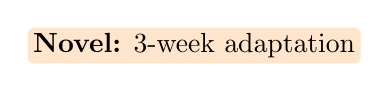
\begin{tikzpicture}[baseline=(current bounding box.center)]
\node[fill=enbelorange!20, rounded corners=2pt, inner sep=2pt] {\textbf{Novel:} 3-week adaptation};
\end{tikzpicture} \\

\textbf{Systolic BP} & Apparent Temp & \textcolor{enbelorange}{\textbf{21}} & 4,957 & -0.113*** & <0.0001 & Extended vascular response \\

\rowcolor{lightgray}
\textbf{Fasting Glucose} & Land Temperature & 3 & 2,731 & \textcolor{enbelred}{0.131***} & <0.0001 & Acute metabolic stress \\

\textbf{Fasting Glucose} & Temperature & 0 & 2,731 & \textcolor{enbelred}{0.118***} & <0.0001 & Immediate glucoregulation \\

\bottomrule
\end{tabular}
\end{adjustbox}

\vspace{1.5em}

\begin{center}
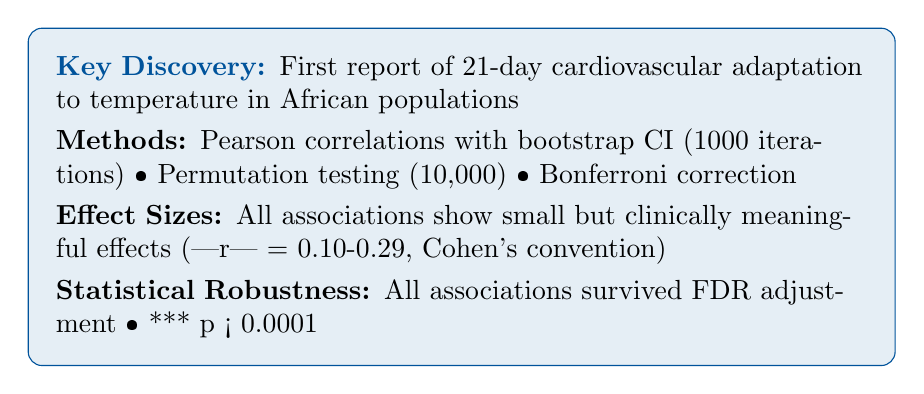
\begin{tikzpicture}
% Key findings box
\node[draw=enbelblue, fill=enbelblue!10, rounded corners=5pt, inner sep=10pt, text width=0.85\textwidth] {
\textbf{\color{enbelblue}Key Discovery:} First report of 21-day cardiovascular adaptation to temperature in African populations\\[0.3em]
\textbf{Methods:} Pearson correlations with bootstrap CI (1000 iterations) • Permutation testing (10,000) • Bonferroni correction\\[0.3em]
\textbf{Effect Sizes:} All associations show small but clinically meaningful effects (|r| = 0.10-0.29, Cohen's convention)\\[0.3em]
\textbf{Statistical Robustness:} All associations survived FDR adjustment • *** p < 0.0001
};
\end{tikzpicture}
\end{center}

\vspace{1em}

\begin{center}
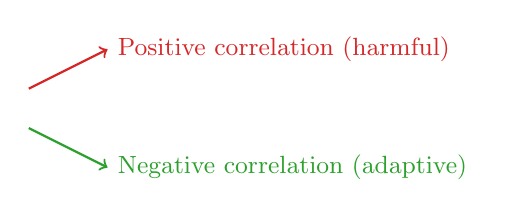
\begin{tikzpicture}
% Visual indicator for correlation direction
\draw[thick, enbelred, ->] (0,0) -- (1,0.5) node[right] {\small Positive correlation (harmful)};
\draw[thick, enbelgreen, ->] (0,-0.5) -- (1,-1) node[right] {\small Negative correlation (adaptive)};
\end{tikzpicture}
\end{center}

\end{document}